% -*- TeX-master: "../dipole_ilya_paper.tex" -*-
\newpage
\section{Dipole Transition}
\label{sec:dipole-transition}

\noindent Finally we characterize  the dipole moment of the
twin qubit for between the  lowest two states, \iket{1} and
\iket{2}.  Microwaves in the  transmission line, carrying a
voltage  $  V_{mw}=   \iabs{V_{mw}}\cos(\omega_{21  }t)  $,  are
coupled via  capacitor C$_{\text{coupling}}$ to  the qubit,
inducing  a charge  $ Q_{2}=C_{\text{coupling}}V_{mw}  $ on
island 2. \iket{1}~\ilra~\iket{2} transitions stimulated by
this    driving,    set    up   a    qubit    voltage    of
$ \delta V_2 = \ibra{1}\hat{V}_{20}\iket{2} $ between the ground
island and island 2 and  hence draw an electrostatic energy
related to the strength of the drive $\Omega$
\begin{equation}
  \label{eq:dipoleEnergy}
  \begin{aligned}
    \delta V_{2}Q_{2} & = \ibra{1}\hat{V}_{20}\iket{2} C_{\text{coupling}}\iabs{V_{mw}}\cos(\omega_{21}  t) \\
    & = \hbar\Omega\cos(\omega_{21}t).
  \end{aligned}
\end{equation}

\noindent        Thus,       the        evaluation       of
$         \ibra{1}\hat{V}_{20}\iket{2}          =         $
$  \ibra{1}\frac{E_{C}}{2  \iabs{e}(1+\alpha)}\left[\hat{n}_1  +
  2\hat{n}_2 +\hat{n}_3\right]\iket{2}$  gives, up  to some
constants  of proportionality,  the coupling  strength that
can be  achieved with  the twin  qubit system  at different
values of the magnetic field.

To  quantitatively  compare  coupling strength  with  other
types of flux qubit  geometries, we re-express this voltage
element through flux:
\begin{equation}
  \label{eq:dipole_voltage_7}
  \begin{aligned}
    \ibra{1}\hat{V}_2 \iket{2} & =  \frac{d}{dt}\ibra{1}\hat{\Phi}\iket{2}\\
    & = \frac{d}{dt}\left[\left(e^{i\omega_{21}t/2}\ibra{1}\right) \hat{\Phi}\left(e^{+i\omega_{21}t/2}\iket{2}\right)\right]\\
    & = {i\omega_{21}\beta\Phi_0},
  \end{aligned}
\end{equation}

\noindent  where  we have  used  the  free evolution  of  a
2-level  system,  $ U(t)=e^{-i  \frac{\mathcal{H}}{\hbar}t}  $,
$ \mathcal{H}  = -\frac{\hbar\omega_{21}}{2}\sigma_z  $, to draw  out the
time-dependent phases  in the  second line  of calculation.
$\beta  = {\ibra{1}\hat{\Phi}\iket{2}}/{\Phi_0}  $ is  the normalized
coupling constant, that can be compared across geometries.

In Fig.~\ref{fig:fig5},  $\beta$ is  compared between  our twin
qubit   and  a   4-JJ   flux   qubit  \cite{honigl2018}   .
Irrespective of  the energies used in  the simulations, the
twin qubit always has a  local maximum of coupling strength
at                     degeneracy                    points
$ \Phi  = (n+\frac{1}{2})\Phi_0,  n\in\mathbb{Z} $, while  the 4-JJ
coupling strength  goes to  zero. Earlier we  discussed the
benefits of operating qubits  near degeneracy points, where
there is a low magnetic  field sensitivity.  The twin qubit
has  the  feature   of  supporting  \iket{1}\ilra  \iket{2}
transitions at  these optimal working points  - transitions
which are forbidden for other geometries.

\begin{figure}[h]
  \centering \includegraphics[height=5cm]{fig5}
  \caption{\small \textbf{Dipole  transition spectrum:} The
    element $  \ibra{1}\hat{V}_{20}\iket{2} $  is evaluated
    using the flux-dependent eigenstates \iket{1}, \iket{2}
    of the  system's Hamiltonian and normalized to $\beta=\frac{\ibra{1}\hat{V}_2  \iket{2}}{i\omega_{21}\Phi_0}$. Plotted is the absolute magnitude $\iabs{\iabs{\beta}}$, which carries real and imaginary components. For the twin qubit we use the $ \iunit{E_J =  91.0}{GHz}, \iunit{E_C  = 13.50}{GHz}, \iunit{\alpha  = 1.023}{},  \iunit{\eta =
      1.011}{} $ found earlier in the paper, while for the 4-JJ flux qubit we use $ E_{C} = \iunit{20}{GHz}, E_J=\iunit{30}{GHz}, \alpha=0.45 $. The operating regions the qubits lie around degeneracy points $  \Phi =  (n+\frac{1}{2})\Phi_0,  n\in\mathbb{Z}  $, where the 4-JJ flux qubit has a forbidden \iket{1} \ilra \iket{2} transition, signified by a vanishing $\beta$.
    \label{fig:fig5}}
\end{figure}

% \begin{equation}\label{eqn:goldenRule}
%                                 \frac{1}{T_{21}}                              =
%                                 %                                 \frac{1}{Z_0}\hbar\omega_{21}\frac{\iabsSquared{\bra{2}T\iket{1}}}{\hbar^2}.
% \end{equation}

% \noindent The  kinetic term $ T  $ plays the role  of the
% dipole operator for this transition and is evaluated with
% the  eigenstates \iket{1},  \iket{2} of  the Hamiltonian.
% Highest   transition  rates   are  achieved   around  the
% degeneracy                                        biases,
% $   \varphi_{\text{ext}}  =   (2n+1)\pi,   n\in\mathbb{Z}  $,   see
% Fig.~\ref{fig:dipole_transition}.   This  region is  thus
% favourable  for  quick  state  operations  with  external
% driving fields.
 
% \begin{figure}
%   \centering 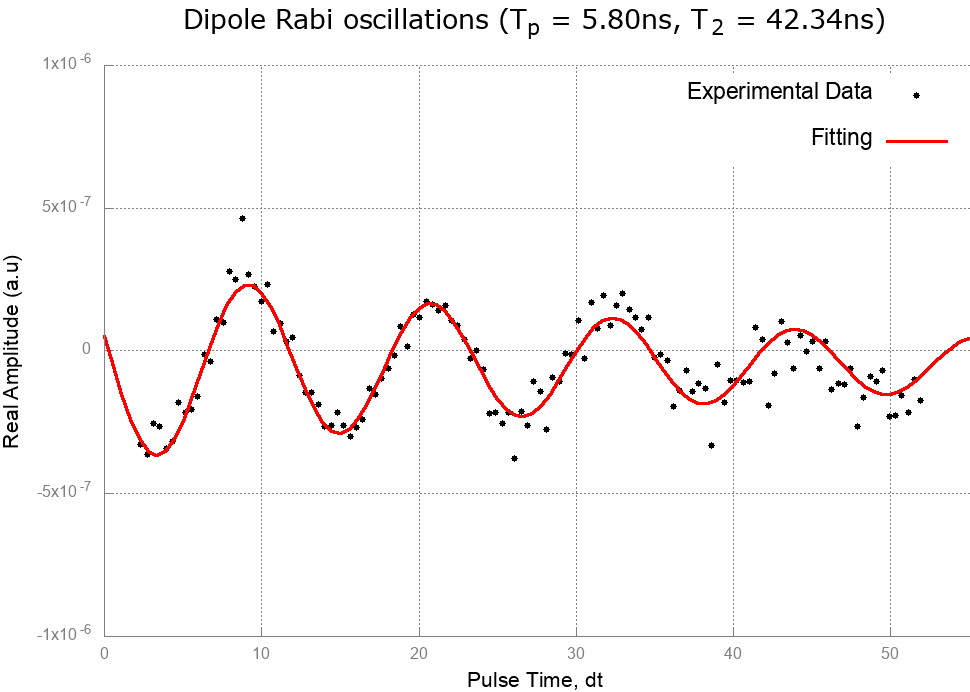
\includegraphics[height=6.5cm]{figure5.png}
 % 	\caption{The dipole transition rate $ \Gamma $ is proportional to the dipole transition element $ \bra{2}T\ket{1} $, where $ T $ is the charge operator responsible for the transition, and $ \iket{1} $ and \iket{2} are the eigenstates of the system. %There is strong transition between the levels at the turning point in magnetic flux, $ \Phi = (n+\frac{1}{2})\Phi_0, n\in\mathcal{Z} $.
 %  \label{fig:dipole_transition}}
 % \end{figure}

%%% Local Variables:
%%% mode: latex
%%% TeX-master: "../dipole_ilya_paper"
%%% End:
